\documentclass[12pt]{article}
\usepackage[letterpaper,top=2.54cm,bottom=2.54cm,left=2.54cm,right=2.54cm,marginparwidth=1.75cm]{geometry}
%% Language and font encodings
\usepackage[english]{babel}
\usepackage[utf8x]{inputenc}
\usepackage[T1]{fontenc}
\usepackage{graphicx}
\usepackage{subcaption}
\usepackage{mwe}
\usepackage{float}
\usepackage{amsmath}
\usepackage{multicol}
\usepackage[colorinlistoftodos]{todonotes}
\usepackage[colorlinks=true, allcolors=blue]{hyperref}
\usepackage{listings}
\usepackage{mathptmx}
\usepackage{color}
\usepackage{amsmath}
\usepackage{amssymb}
\usepackage{epstopdf}
\usepackage{inputenc}
\usepackage{geometry}
\usepackage{color}
\usepackage[nottoc]{tocbibind}
\usepackage{natbib}
\usepackage{courier}
\usepackage{algorithm}
\usepackage[noend]{algpseudocode}
\usepackage{qtree}
\usepackage{forest}
\usepackage{datetime}

\makeatletter
\def\BState{\State\hskip-\ALG@thistlm}
\makeatother

%% Matlab
\definecolor{mygreen}{RGB}{28,172,0} % color values Red, Green, Blue
\definecolor{mylilas}{RGB}{170,55,241}

\lstset{language=C++,%
    basicstyle=\scriptsize\ttfamily,
    breaklines=true,%
    morekeywords={matlab2tikz},
    keywordstyle=\color{blue},%
    morekeywords=[2]{1}, keywordstyle=[2]{\color{black}},
    identifierstyle=\color{black},%
    stringstyle=\color{mylilas},
    commentstyle=\color{mygreen},%
    showstringspaces=false,%without this there will be a symbol in the places where there is a space
    numbers=left,%
    numberstyle={\tiny \color{black}},% size of the numbers
    numbersep=9pt, % this defines how far the numbers are from the text
    emph=[1]{for,end,break},emphstyle=[1]\color{red}, %some words to emphasise
    emph=[2]{word1,word2}, emphstyle=[2]{style},    
}


\begin{document}
\begin{titlepage}
	\centering
	{\scshape\LARGE Columbia University \par}
	\vspace{1cm}
	{\scshape MECE 4510 Evolutionary Computation and Design Automation\par}
	\vspace{1.5cm}
	{\huge\bfseries Assignment3-Phase A\par}
	\vspace{2cm}
	{\Large\itshape Hanwen Zhao\par}
	{UNI: hz2547\par}
	\vfill
	supervised by\par
	Dr.~Hod \textsc{Lipson}
	\vfill
	Grace Hours Used: 53\\
	Grace Hours Accumulated: 70\\
	Grace Hours Remaining: 113 \\
	\vspace{2cm}
% Bottom of the page
	{\large \today \ \currenttime \par}
\end{titlepage}

\newpage
\section{Result Summary}
\begin{figure}[H]
	\centering
	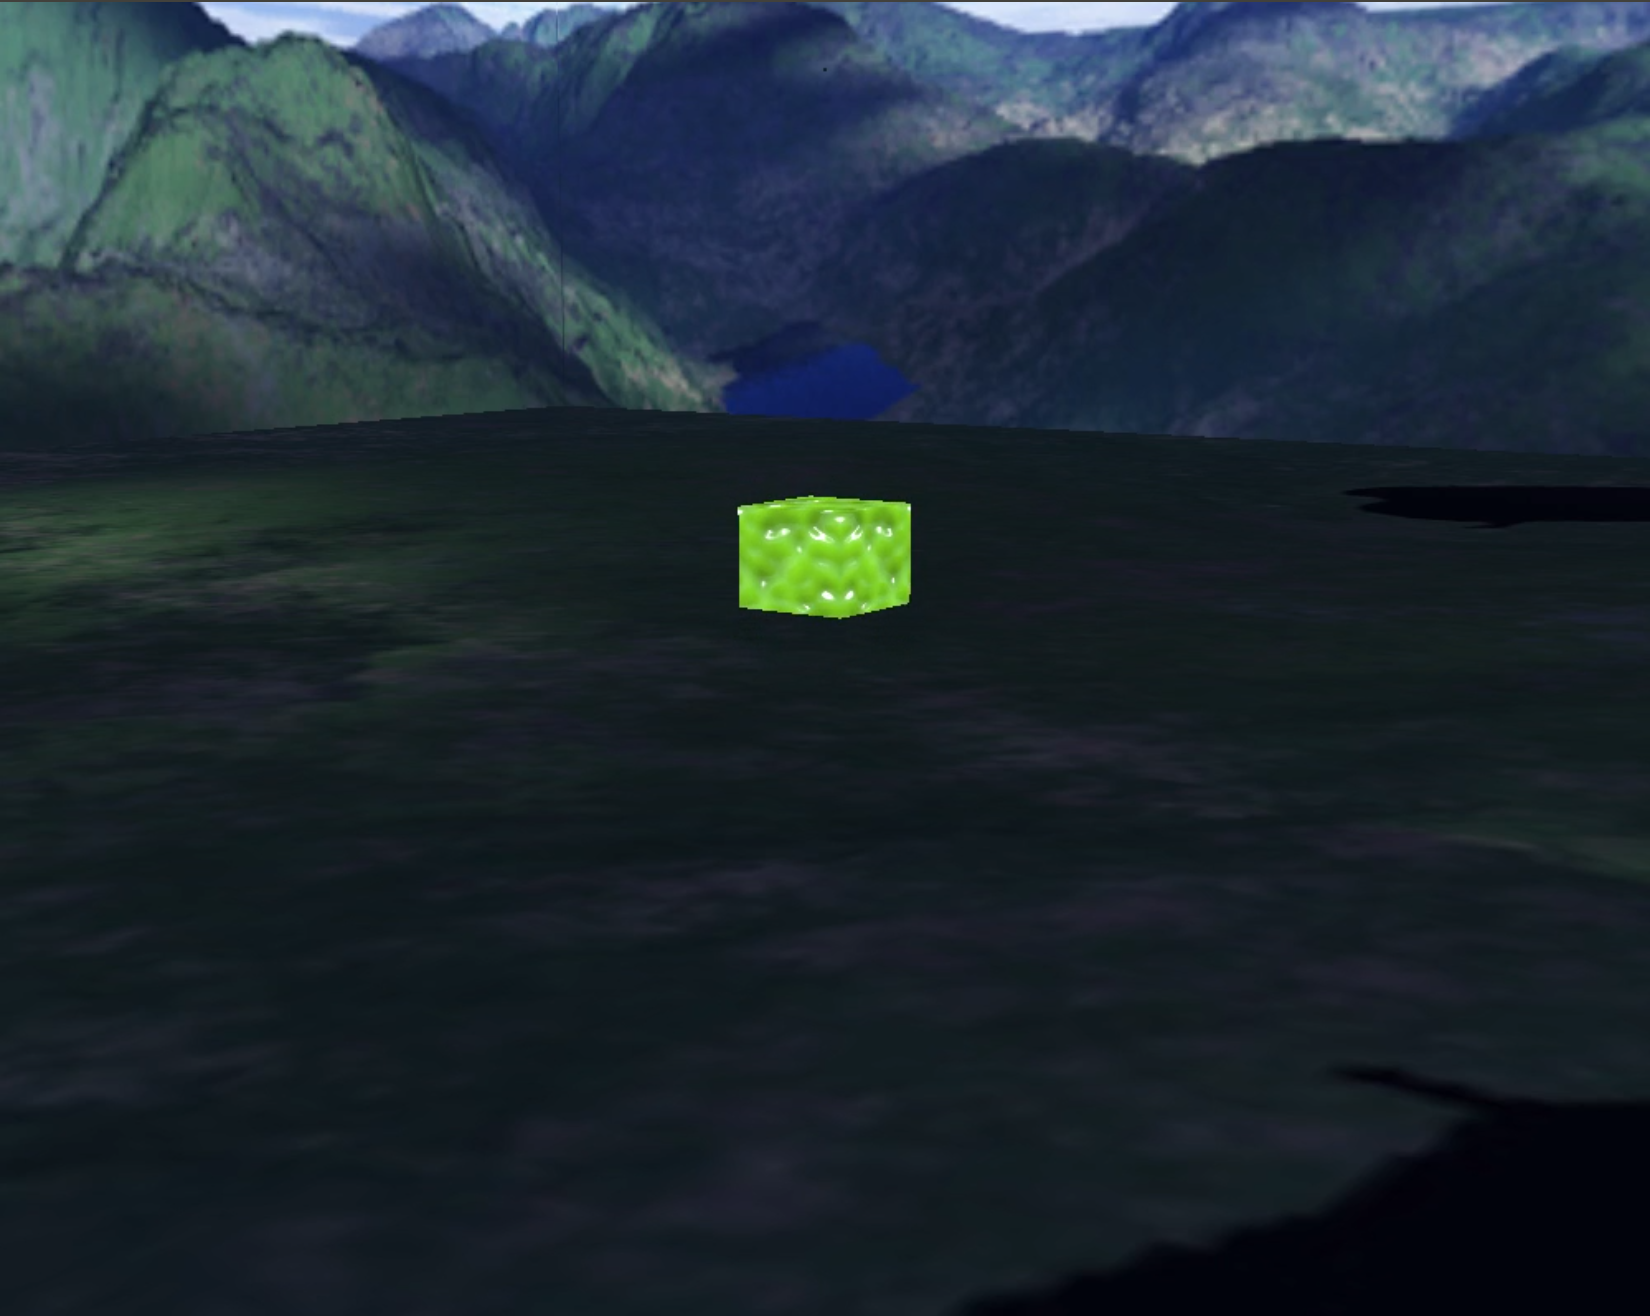
\includegraphics[width=0.5\textwidth]{BouncingCube}
	\caption[]%
	{{\small Bouncing Cube}}    
\end{figure}
url: \url{https://goo.gl/zvWsxR}

\begin{figure}[H]
	\centering
	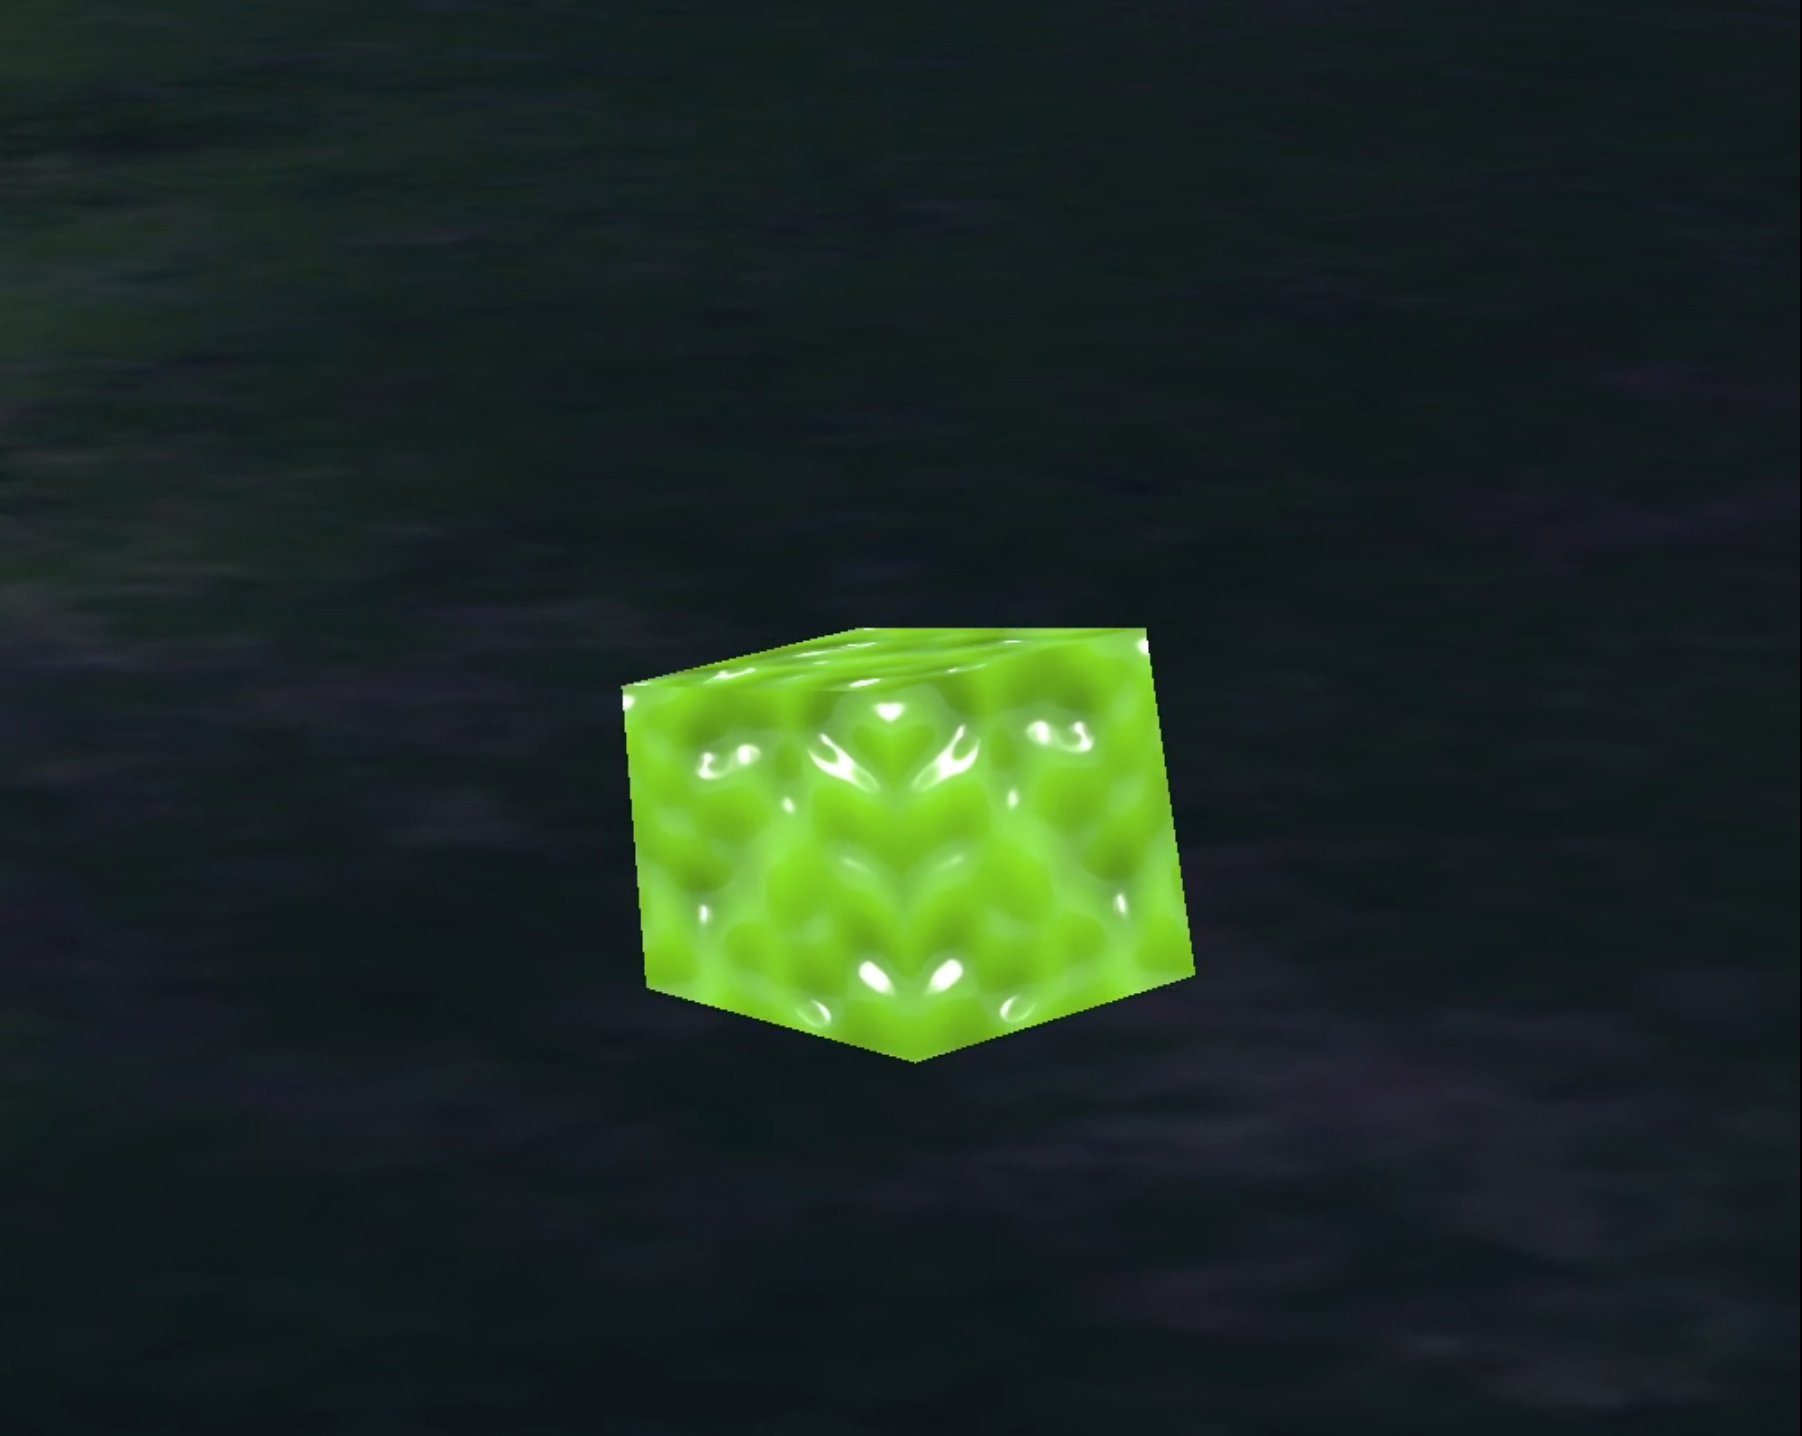
\includegraphics[width=0.5\textwidth]{BreathingCube}
	\caption[]%
	{{\small Breathing Cube}}    
\end{figure}
\noindent
url: \url{https://goo.gl/HaBNAk}


\newpage
\section{Methods}
\subsection{Description of Design}
As the first phase of our final project, we need to create a physics simulator that could simulate a simple cube bouncing on a flat plane and also be able to "breathe" by changing the rest length for the springs.\\
In order to better prepare for the final project, I have decided to use C++ and OpenGL since they are much faster than python, which we can benefit for the simulation time for the final project.\\
The physics simulator is relevant straightforward, the following are my parameters for both bouncing cube and breathing cube.
\subsubsection{Bouncing Cube}
\begin{itemize}
\setlength\itemsep{0em}
\item mass = 0.1 kg
\item length = 0.1 kg
\item gravity = 9.81 N/kg
\item time step = 0.001 s
\item spring constant = 1000 N/m
\item ground restoration constant = 10000 N/m
\item dampening constant = 0.999
\end{itemize}

\subsubsection{Breathing Cube}
\begin{itemize}
\setlength\itemsep{0em}
\item mass = 0.1 kg
\item length = 0.1 kg
\item gravity = 9.81 N/kg
\item time step = 0.001 s
\item spring constant = 100 N/m
\item ground restoration constant = 10000 N/m
\item dampening constant = 0.999
\end{itemize}

\subsection{Analysis}
Overall everything goes smoothly, however writing OpenGL is somewhat difficult. In addition, for final project writing the evolutionary algorithm in C++ might take longer time. A way to get around is to use ROS to get communication between Python and C++.


\newpage
\section{Performance}
\subsection{Performance Plots}
\begin{figure}[H]
	\centering
	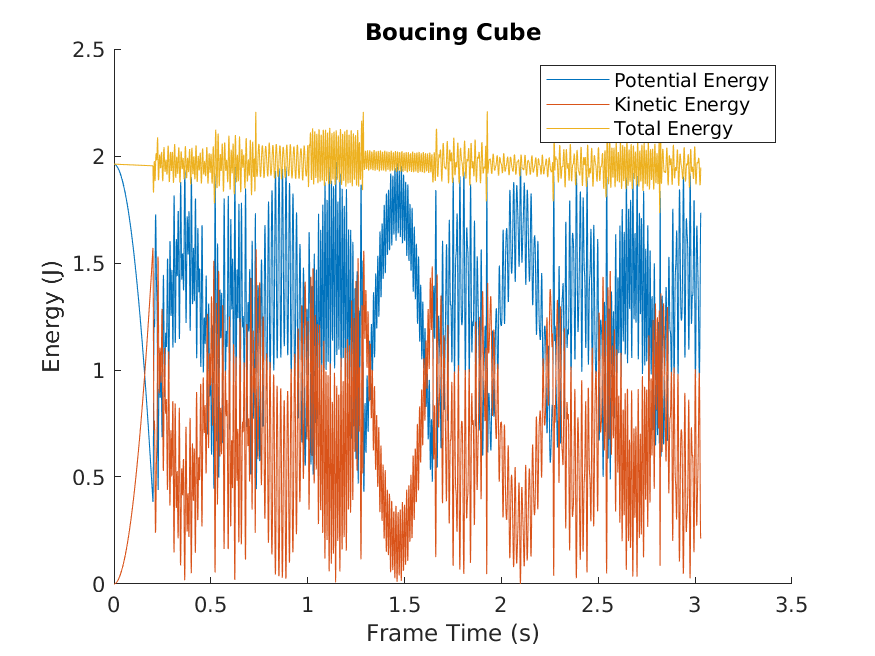
\includegraphics[width=0.7\textwidth]{BouncingCubeEnergy}
	\caption[]%
	{{\small 38047 spring evaluations/second}}    
\end{figure}
\begin{figure}[H]
	\centering
	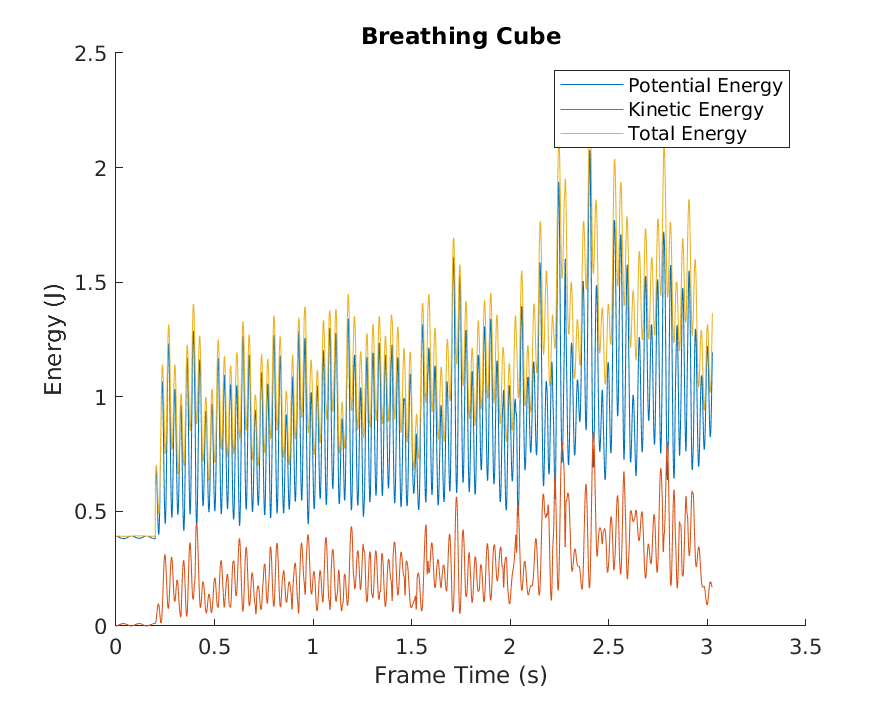
\includegraphics[width=0.7\textwidth]{BreathingCubeEnergy}
	\caption[]%
	{{\small 36857 spring evaluations/second}}    
\end{figure}
\newpage
\section{Additonal Tasks}
\subsection{Bouncing with Spin}
\begin{figure}[H]
	\centering
	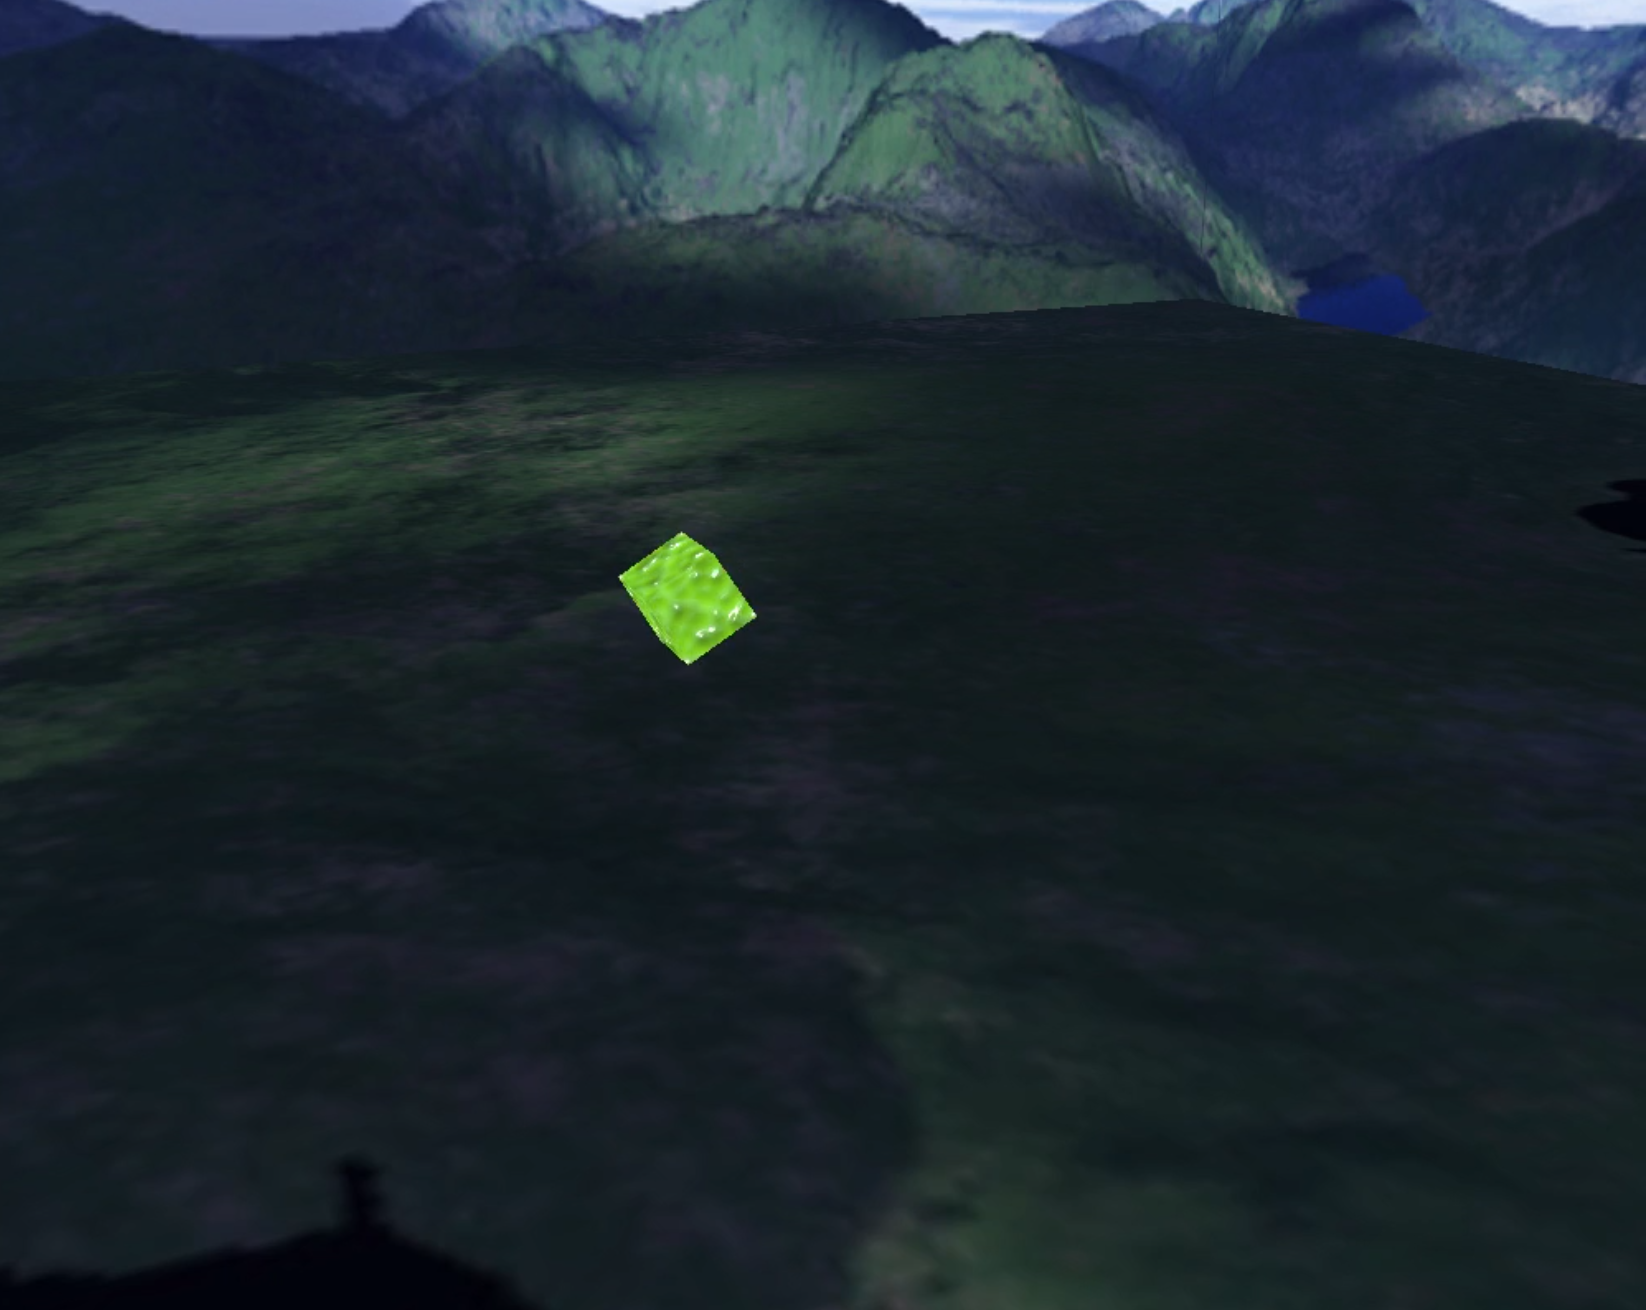
\includegraphics[width=0.5\textwidth]{BouncingWithSpin}
	\caption[]%
	{{\small Bouncing Cube with Spin}}    
\end{figure}
url: \url{https://goo.gl/Zvn3qs}

\subsection{Bouncing with Dampening}
\begin{figure}[H]
	\centering
	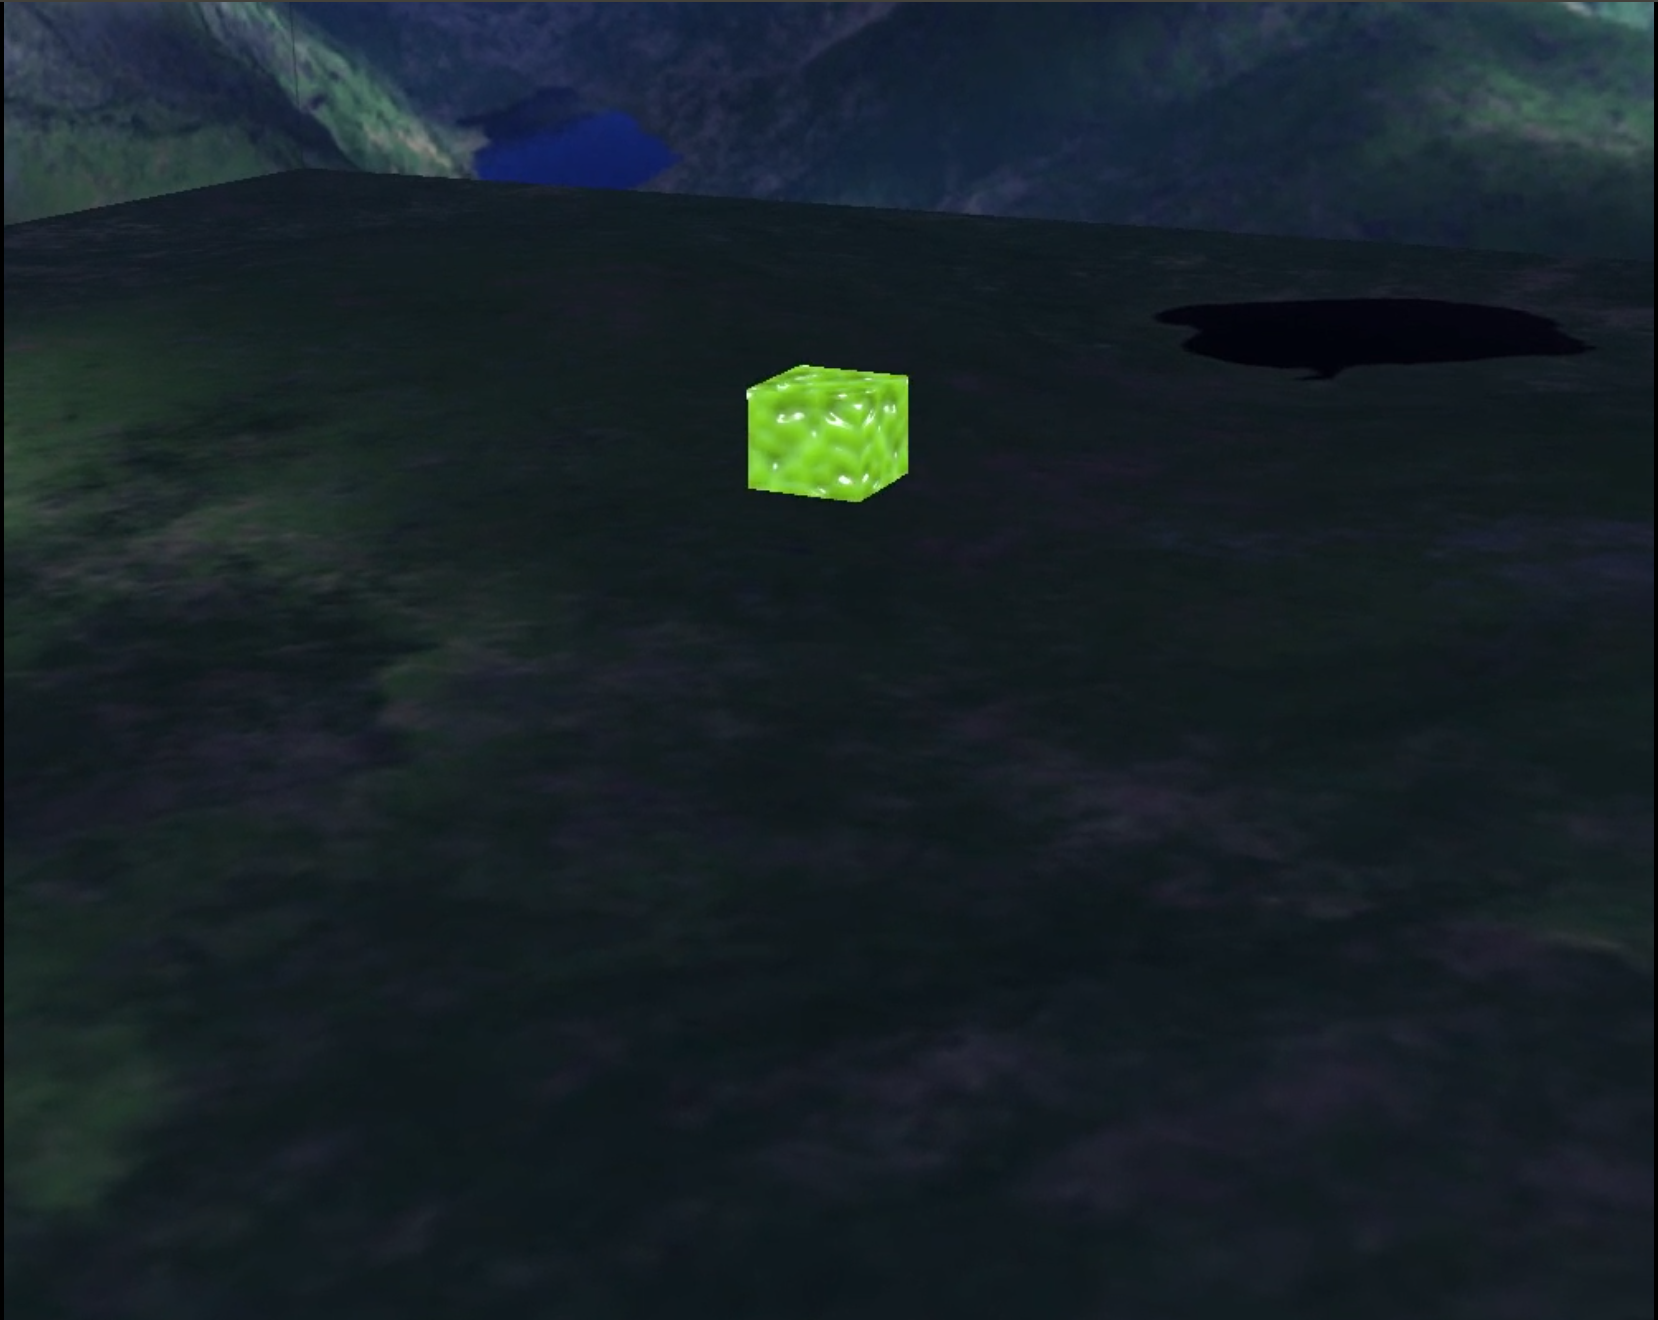
\includegraphics[width=0.5\textwidth]{BouncingWithDampening}
	\caption[]%
	{{\small Bouncing Cube with Dampening}}    
\end{figure}
url: \url{https://goo.gl/U3QD3Z}

\subsection{Newtonian Friction}
\begin{figure}[H]
	\centering
	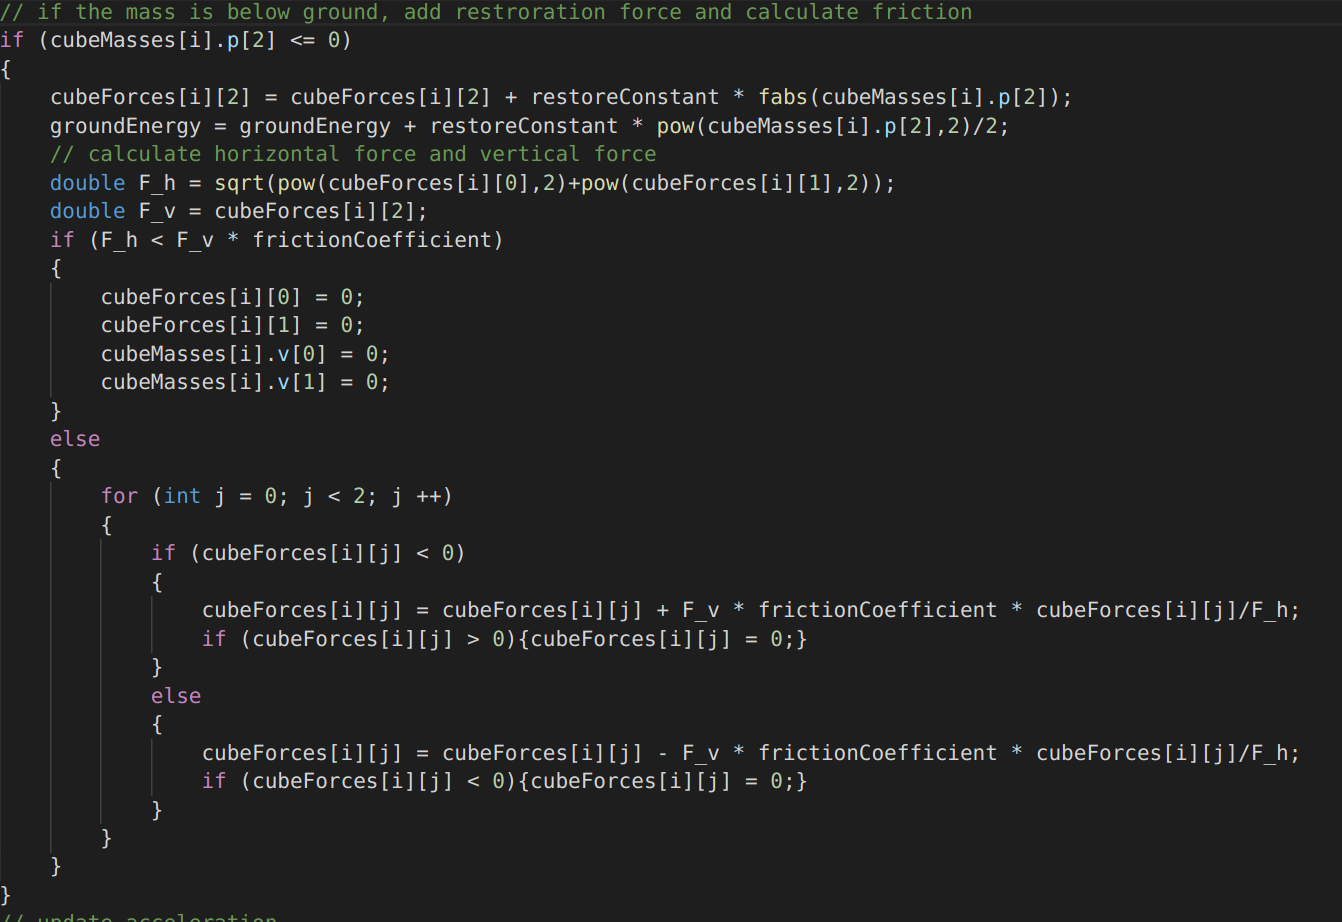
\includegraphics[width=0.5\textwidth]{frictionCode}
	\caption[]%
	{{\small Line 298 - 329}}    
\end{figure}

\subsection{Grounded Node}
\begin{figure}[H]
	\centering
	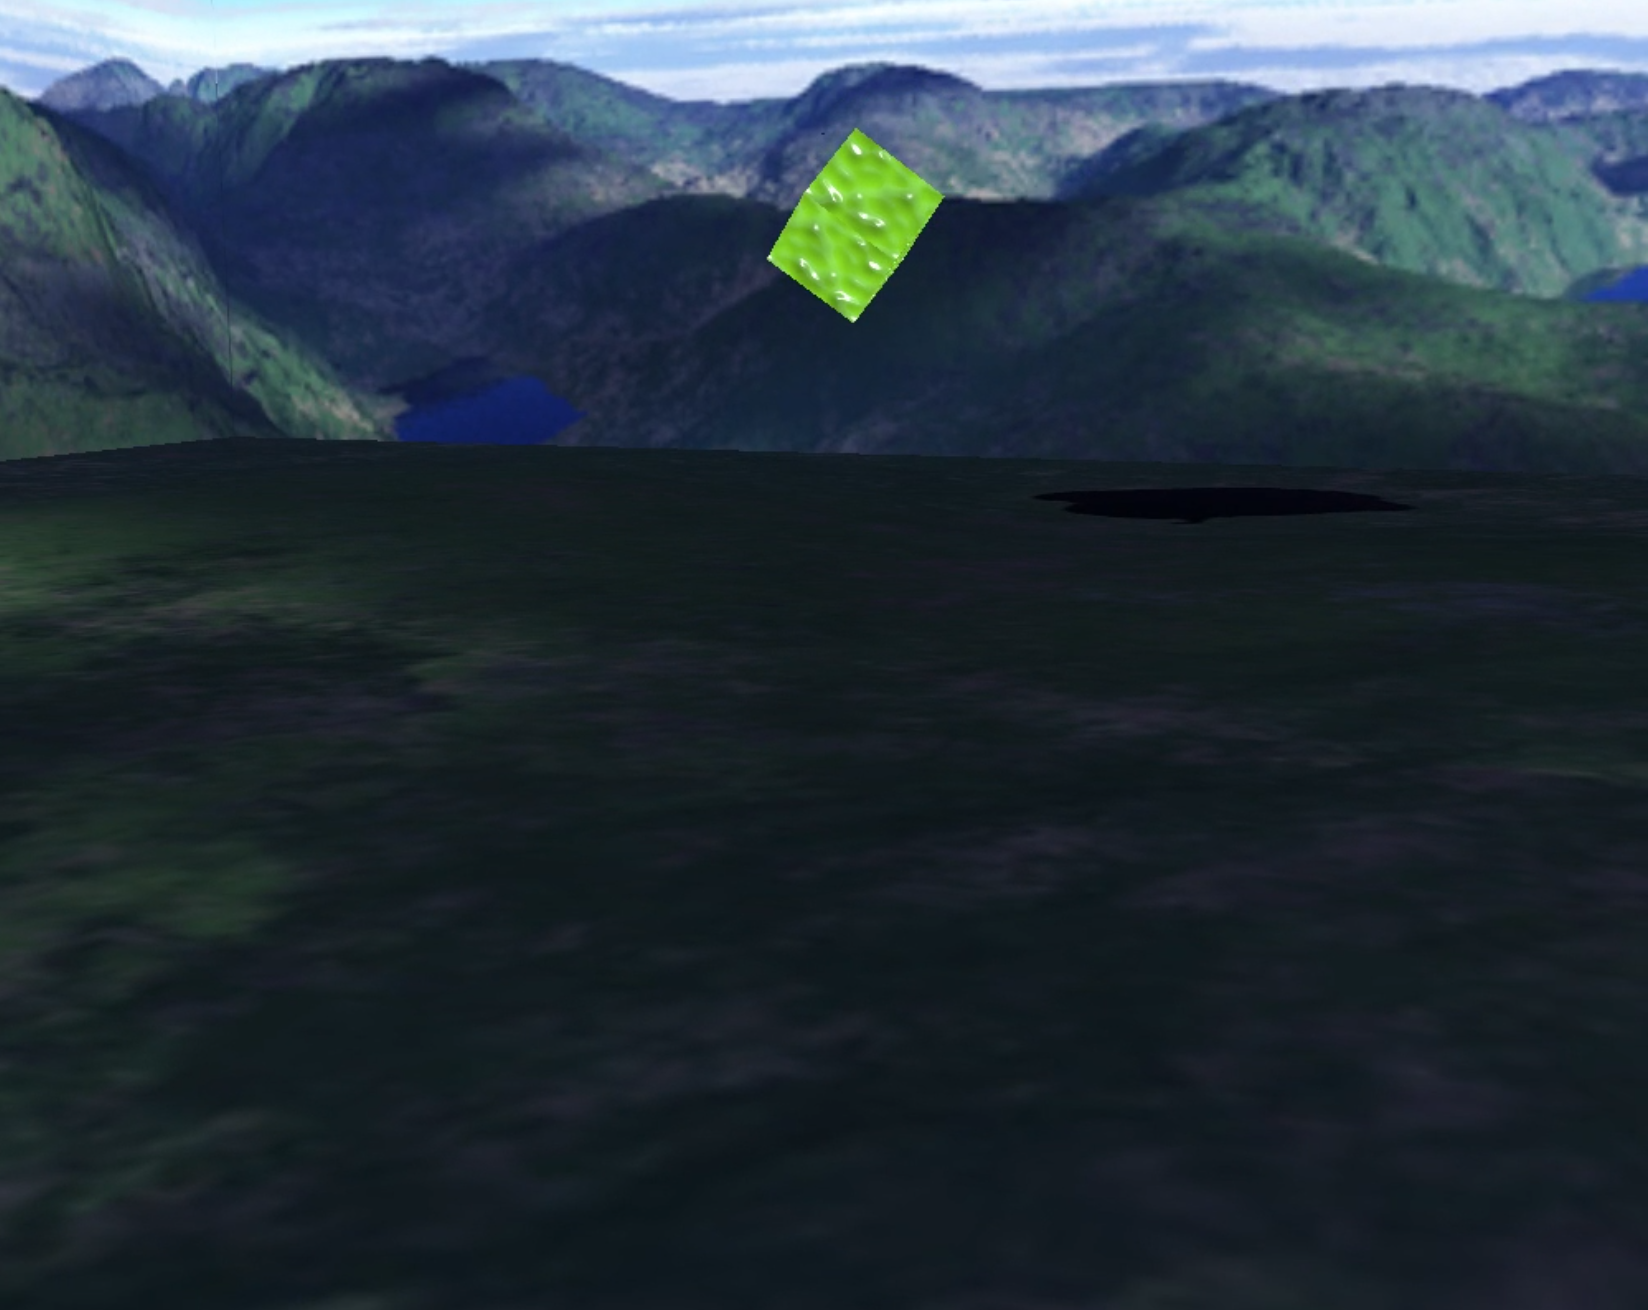
\includegraphics[width=0.5\textwidth]{groundedNode}
	\caption[]%
	{{\small Grounded Node}}    
\end{figure}
url: \url{https://goo.gl/T13dHs}




\newpage
\section{Appendix}
\lstinputlisting{HW3.cpp}



\end{document}